% !TEX program = pdflatex
\documentclass[a4paper,11pt]{article}
\usepackage[a4paper]{geometry}
%
%
\usepackage{graphicx}
\usepackage{amssymb,amsmath, amsthm}
\usepackage{mathrsfs}
\usepackage{bbm,bbold}
\usepackage{todonotes}
\usepackage{lineno}
\usepackage{enumitem}
\usepackage{booktabs}
\usepackage{caption}
\usepackage{subcaption}
\usepackage{wrapfig}

\usepackage{comment}

%%%%% THEOREM ENVIRONMENTS
\theoremstyle{plain}
\newtheorem{theorem}{Theorem}
\newtheorem{proposition}[theorem]{Proposition}
\newtheorem{lemma}[theorem]{Lemma}
\newtheorem*{lemma*}{Auxiliary Lemma}
\newtheorem{observation}[theorem]{Observation}
\newtheorem{corollary}[theorem]{Corollary}
\newtheorem{fact}[theorem]{Fact}
\newtheorem{conjecture}{Conjecture}
\newtheorem{problem}[theorem]{Problem}
\newtheorem*{conj1}{Conjecture 1}
\newtheorem*{conj2}{Conjecture 2}
\newtheorem*{conj1k2k}{Conjecture 1'}%$_{(k\hookrightarrow 2k)}$}

\theoremstyle{definition}
\newtheorem{definition}[theorem]{Definition}
\newtheorem{remark}[theorem]{Remark}
\newtheorem{remarks}[theorem]{Remarks}
\newtheorem*{acknowledgements}{Acknowledgements}
\newtheorem{example}[theorem]{Example}

\theoremstyle{remark}
\newtheorem{claim}{Claim}

%%% BOLD MATH
\newcommand{\myboldmath}[1]{\mathbbm{#1}}
\newcommand{\R}{\myboldmath{R}}
\newcommand{\G}{\myboldmath{G}}
\newcommand{\Q}{\myboldmath{Q}}
\newcommand{\N}{\myboldmath{N}}
\newcommand{\Z}{\myboldmath{Z}}
\newcommand{\F}{\myboldmath{F}}
\newcommand{\s}{\myboldmath{S}}
\newcommand{\C}{\myboldmath{C}}

\newcommand{\1}{\mathbf{1}}
\newcommand{\E}{\myboldmath{E}}

%%% SIMPLICIAL COMPLEXES AND GRAPHS
\DeclareMathOperator{\st}{st}
\DeclareMathOperator{\lk}{lk}
\newcommand{\bd}{\partial}
\newcommand{\im}{\operatorname{im}}

%%%% OTHER STUFF
\DeclareMathOperator{\supp}{supp}
\newcommand{\up}{\textup{up}}
\newcommand{\down}{\textup{down}} 


\begin{document}
\linenumbers

%%%%OPENING
\title{Hit and Run and Stuff}
\author{Brian Cohn \and May Szedl\'{a}k}
\begin{titlepage}
\maketitle
\thispagestyle{empty}
%%
\begin{abstract}
The brain must select its control strategies among an infinite set of possibilties, thereby solving an optimization problem. 
While this set is infinite and lies in high dimensions, it is bounded by kinematic, neuromuscular, and anatomical constraints, within which the brain must select optimal solutions. 
We use data from a human index finger with 7 muscles, 4DOF, and 4 output dimensions. For a given force vector at the endpoint, the feasible activation space is a 3D convex polytope, embedded in the 7D unit cube.
It is known that explicitly computing the volume of this polytope can become too computationally complex in many instances. 
We generated random points in the feasible activation space using the Hit-and-Run method, which converged to the uniform distribution. 
After generating enough points, we computed the distribution of activation across each muscle, shedding light onto the structure of these solution spaces- rather than simply exploring their maximal and nimimal values. 
We also visualize the change in these activation distributions as we march toward maximal feasible force production in a given direction. 
Using the parallel coordintes method, we visualize the connection between the muscle activations. Once can then explore the feasible activation space, while constraining certain muscles.
Although this paper presents a 7 dimensional case of the index finger, our methods extend to systems with up to at least 40 muscles. We challenge the community to map the shapes distributions of each variable in the solution space, thereby providing important contextual information into optimization of motor cortical function in future research.
\end{abstract}
%%
\end{titlepage}
%%%%

%%%%ARTICLE
\section{Author Summary}
brian is a phd student\\
may is a phd student\\
bernt, komei, and francisco are professors

\section{INTRODUCTION}

Muscle redundancy is the term used to describe the underdetermined nature of neural control of musculature.
The classical notion of muscle redundancy  proposes that, faced with an infinite number of possible muscle activation patterns for a given task, the nervous system uses optimization to select a given specific solution.
Here, each of the $N$ muscles represents a dimension of control, and a muscle activation pattern is a point in $\mathbb{R}^N$ \cite{Valero-Cuevas1998Large}.
Thus researchers often seek to infer the optimization approach and the cost functions the nervous system likely utilizes to find the points in activation space to produce natural behavior \cite{Chao1978Graphical,Prilutsky2000Muscle,scott2004optimal,todorov2002optimal,crowninshield1981physiologically,higginson2005simulated}. 


Implicit in these optimization procedures is the notion that there exists a well structured set of feasible solutions. Thus several of us have focused on describing and understanding those high-dimensional subspaces  embedded in $\mathbb{R}^N$ \cite{kutch2011muscle,kutch2012challenges,sohn2013cat_bounding_box,Valero-Cuevas1998Large,Valero-Cuevas2015high-dimensional}.

For the case of muscle redundancy for submaximal and static force production with a limb,  the problem is phrased as one of computational geometry: find the convex polytope of feasible muscle activations given the mechanics of the limb and the constrains of the task \cite{avis1992Pivoting,Valero-Cuevas1998Large,Valero-Cuevas2009mathematical,Valero-Cuevas2015high-dimensional}.  This convex polytope is called the \emph{feasible activation set}. To date, the structure of this high-dimensional polytope is inferred by its bounding box  \cite{kutch2011muscle,sohn2013cat_bounding_box,Valero-Cuevas2015high-dimensional}.  But the bounding box of a convex polytope will always overestimate its volume, and lose the details of its shape.  Empirical dimensionality-reduction methods have also been used to calculate a basis vectors for such subspaces \cite{Clewley2008Estimating,davella2005shared,krishnamoorthy2003muscle}. But those basis  vectors only provide a description of the dimension, orientation, and aspect ratio of the polytope, but not of its boundaries or internal  structure.

Here we present a novel application of the well-known Hit-and-Run algorithm \cite{smith1984efficient} to describe the internal structure of these high-dimensional feasible activation sets. We apply our technique to a schematic example with three muscles to describe the method, and then use realistic model of an index finger with seven muscles and four joints \cite{Valero-Cuevas1998Large}.
\section{Materials and Methods}

% TODO Insert the J and R matrices, and show their multiplication
% Sample Calculation X.

% TODO Insert the F_o Vector
% Table X.


% TODO Insert the A matrix, ith full muscle names
% Table X. Each column represents a wrench generators (with each dimension in Newtons). The muscle is modeled such that full activation would produce the column of forces and torque at the fingertip.


\subsection{Data and Samples}
We began with an index finger of a healthy human (male) right hand, which was taken from []. Dissected by []. Experimental forces from []. IUPAC licenses and other important facts. Measurements were made with a ruler, with $\pm x$.
The moment arm matrix, $R$, which contains the leverage of each tendon's insertion points across each joint, was measured by doing [], [] ,and then []. The Jacobian, $J$, which represents the effect of rotation at each DOF on each component of endpoint wrench, was measured with a [], by [], with precision of $\pm x$. The force-naught vector, $F_0$, which contains the tendon force at maximal isometric contration (MIC) for each muscle, was taken in the [same or different] posture, with a [] measuring device, with precision of $\pm x$.

\subsection{Polytope representation of the feasible activation space}
Exact volume calculations for polygons can only be done in reasonable time in up to 10 dimensions \cite{Dyer2, Khachiyan, Khachiyan2}. We therefore use the so called Hit-and-Run approach, which samples a series of points in a given polygon. Given the points for a feasibale activation space, this method gives us a deeper understanding of its underlying structure. 
\subsection{Hit-and-Run}
In this section we introduce the Hit-and-Run algorithm used for uniform sampling in a convex body $K$, was introduced by Smith in 1984 \cite{Smith}. The mixing time is known to be $\mathcal{O}^*(n^2R^2/r^2)$, where $R$ and $r$ are the radii of the inscribed and cicumscribed ball of $K$ respectively \cite{Dyer, Lovasz}. I.e., after $\mathcal{O}^*(n^2R^2/r^2)$ steps of the Hit-and-Run algorithm we are at a uniformly at random point in the convex body. 
In the case of the muscles of a limb, we are interested in the polygon $P$ that is given by the set of all possible activations $\textbf{a} \in \mathbb{R}^n$ that satisfy
\[\textbf{f} = A\textbf{a}, \textbf{a} \in [0,1]^n,\]
where $\textbf{f} \in \mathbb{R}^m$ is a fixed force vector and $A = J^{-T}RF_m \in \mathbb{R}^{m \times n}$. $P$ is bounded by the unit $n$-cube since all variables $a_i$, $i \in [n]$ are bounded by 0 and 1 from below, above respectively.
Consider the following $1 \times 3$ example.
\begin{align*}
&1 = \frac{10}{3}a_1 - \frac{53}{15}a_2 + 2a_3 \\
&a_1, a_2, a_3 \in [0,1],
\end{align*}
the set of feasible activations is given by the shaded set in Figure \ref{fig_hr}.

\begin{figure}[ht]
   \begin{center}
    \includegraphics[width=0.25\textwidth]{feasibleactivation.png}
  \end{center}
  \caption{Feasible Activation}
  \label{fig_hr}
\end{figure}

The Hit-and-Run walk on $P$ is defined as follows (it works analogously for any convex body). 
\begin{enumerate}
\item Find a given starting point $\textbf{p}$ of $P$ (Figure \ref{fig_hr1}) .
\item Generate a random direction through $\textbf{p}$ (uniformly at random over all directions) (Figure \ref{fig_hr2}).
\item Find the intersection points of the random direction with the $n$-unit cube (Figure \ref{fig_hr3}).
\item Choose the next point of the sampling algorithm uniformly at random from the segment of the line in $P$ (Figure \ref{fig_hr4}). 
\item Repeat from $(b)$ the above steps with the new point as the starting point .
\end{enumerate}


\begin{figure}
        \centering
        \begin{subfigure}[b]{0.25\textwidth}
                \includegraphics[width=\textwidth]{HR2.png}
                 \caption{Inner Point}
      						\label{fig_hr1}
        \end{subfigure} \hspace{0.5cm}
        \begin{subfigure}[b]{0.25\textwidth}
                \includegraphics[width=\textwidth]{HR3.png}
                \caption{Direction}
      					\label{fig_hr2}
        \end{subfigure} \\
        \begin{subfigure}[b]{0.25\textwidth}
                \includegraphics[width=\textwidth]{HR4.png}
                 \caption{Endpoints}
      					\label{fig_hr3}
        \end{subfigure} \hspace{0.5cm}
        \begin{subfigure}[b]{0.25\textwidth}
                \includegraphics[width=\textwidth]{HR5.png}
                \caption{New Point}
      				 \label{fig_hr4}
        \end{subfigure}
        \caption{Hit-and-Run Step}\label{fig:animals}
\end{figure}

%\begin{figure}[ht]
%   \begin{center}
%    \includegraphics[width=0.25\textwidth]{HR1.png}
%      \caption{Inner Point}
%      \label{fig_hr1}
%    \includegraphics[width=0.25\textwidth]{HR2.png}
%    \caption{Direction}
%      \label{fig_hr2}
%    \includegraphics[width=0.25\textwidth]{HR3.png}
%    \caption{Endpoints}
%      \label{fig_hr3}
%    \includegraphics[width=0.25\textwidth]{HR4.png}
%    \caption{New Point}
%      \label{fig_hr4}
%  \end{center}
%\end{figure}

\begin{figure}[ht]
   \begin{center}
    \includegraphics[width=0.25\textwidth]{uniform.png}
      \caption{Uniform Distribution}
      \label{fig_hr5}
  \end{center}
\end{figure}


The implementation of this algorithm is straight forward except for the choice of the random direction. How do we sample uniformly at random (u.a.r.) from all directions in $P$? Suppose that $\textbf{q}$ is a direction in $P$ and $p \in P$. Then by definition of $P$, $\textbf{q}$ must satisfy $\textbf{f} = A(\textbf{p}+\textbf{q})$. Since $\textbf{p} \in P$, we know that $\textbf{f} = A\textbf{p}$ and therefore 
\[\textbf{f} = A(\textbf{p} + \textbf{q}) = \textbf{f} + A\textbf{q}\]
and hence
\[A\textbf{q} = 0.\]

We therefore need to choose directions uniformly at random from all directions in the vectorspace 
\[V = \{\textbf{q} \in \mathbb{R}^n | A\textbf{q} = 0\}.\]

As shown by Marsaglia this can be done as follows \cite{Marsaglia}.

\begin{enumerate}
\item
Find an orthonormal basis $b_1, \dots, b_r \in \mathbb{R}^{n}$ of $A\textbf{q} =0$.
\item
Choose $(\lambda_1, \dots, \lambda_r) \in \mathcal{N}(0,1)^n$ (from the Gaussian distribution).
\item
$\sum_{i=1}^r \lambda_i b_i$ is a u.a.r.\ direction.
\end{enumerate}

A basis of a vectorspace $V$ is a minimal set of vectors that generate $V$, and it is orthonormal if the vectors are pairwise orthogonal (perpendicular) and have unit length. Using basic linear algebra one can find a basis for $V = \{A\textbf{q} = 0\}$ and orthogonalize it with the well known Gram-Schmidt method (for details see e.g.\ \cite{Robertson}). Note that in order to get the desired u.a.r.\ sample the basis needs to be orthonormal. For the limb case we can safely assume that the rows of $A$ are linearly independent and hence the number of basis vectors is $n-m$.



\begin{figure}
        \centering
        \begin{subfigure}[b]{0.25\textwidth}
                \includegraphics[width=\textwidth]{somebasis.png}
      \caption{Some Basis}
      \label{fig_somebasis}
              \end{subfigure} \hspace{0.5cm}
        \begin{subfigure}[b]{0.25\textwidth}
                \includegraphics[width=\textwidth]{orthobasis.png}
     \caption{Direction}
      \label{Orthonormal Basis}        
      \end{subfigure}
      \caption{Find Orthonormal Basis}\label{fig_basis} 
\end{figure}


\subsection{Mixing Time}
How many steps are necessary to reach a uniformly at random point in the polytope? The theoretical bound $\mathcal{O}^*(n^2R^2/r^2)$ given in \cite{Lovasz} has a very large hidden coefficient ($10^30$) which makes the algorithm almost infeasible in lower dimensions.

These bounds hold for general convex sets. For convex polygons in higher dimensions, experimental results suggest that $\mathcal{O}(n)$ steps of the Hit-and-Run algorithm are sufficient. In particular Emiris and Fisikopoulos paper suggest that $(10 + 10\frac{n})n$ steps are enough to have a close to uniform distribution \cite{Emiris}. In all cases tested, sampling more point did not make accuarcy significantly higher. 

Ge et al.\ showed experimentally that up to about 40 dimensions, ??? random points seem to suffice to get a close to uniform discussion \cite{Ge}. 

Therfore for given output force we execute the Hit-and-Run algorithm 1000 times on 100 points. The experimental results propose that those 1000 points are uniformly distributed on the polygon.

As a additional control, for each muscle we observe that the theoretical upper and lower bound of the feasible activation match the observed corresponding bounds (difference max ??). To find the theoretical upperbound (lowerbound) of a given muscle activation we solve two linear programs maximizing (minimizing)  $a_i$ over the polytope.


%For the upper and lower bounds of the activation we can solve two linear program for each coordinate of $\textbf{a}$ to find the upper and lower bounds of each $a_i$.
%We see that those theoretical bounds match the experimentally obtained bounds.

\subsection{Starting Point}
To find a starting point in 
\[\textbf{f} = A\textbf{a}, \textbf{a} \in [0,1]^n,\]
we only need to find a feasible activation vector. For the hit and run algorithm to mix faster, we do not want the starting point to be in a vertex of the activation space. We use the following standard trick using slack variables $\epsilon_i$.

\begin{equation}\label{eq:LP_r}
\begin{array}{lrcl}
\mbox{maximize} & \sum_{i=1}^n \epsilon_i \\ 
\mbox{subject to} & \textbf{f} &=& A\textbf{a}\\
  & a_i &\in& [\epsilon_i, 1- \epsilon_i], \hspace{5mm} \forall i \in \{1,\dots,n\}  \\
  & \epsilon_i &\geq& 0, \hspace{5mm} \forall i \in \{1,\dots,n\}.  
\end{array}
\end{equation}

This approach can still fail in theory, but this method has the choose $\epsilon_i > 0$ and therefore $a_i \neq 0$ or $1$. Since for all vertices of the feasible activation space lie on the boundary of the $n$-cube, at least $n-m$ muscles must have activation $0$ or $1$. Documentation is included in our supplementary information.

\subsection{Parallel Coordinates: Visualization of the Feasible Activation Space}
Citation
A common way to visualize higher dimensional data is using parallel coordinates. To show our sample set of points in the feasible activation space we draw $n$ parallel lines, which representing the activations of the $n$ muscles. Each point is then represented by connecting their coordinates by $n-1$ lines.


\begin{figure}[ht]
   \begin{center}
    \includegraphics[width=0.5\textwidth]{pc.png}
  \end{center}
  \caption{Feasible Activation}
  \label{fig_pc}
\end{figure}

Using an interactive surface one can now restrict each muscle function to any desired interval, e.g., figure ??.

\textbf{NICE FIGURE OF RESTRICTED PARALLEL COORDINATES}

For the $l_1$, $l_2$ and $l_3$ norm respectively, we added an additional line to represent the corresponding weight. E.g.\ for a given point $\textbf{a} \in \mathbb{R}^n$ we are interested in $\sum_{i=1}^n a_i$, $\sqrt{\sum_{i=1}^n a_i^2}$ and $\sqrt[3]{\sum_{i=1}^n a_i^3}$. As for the muscles one can restrict the intervals of the weight functions, to explore the corresponding feasible activation space. 

\textbf{NICE PICTURE WITH WEIGHTS INCLUDED}
We found the feasible activation set for the task of producing nine different sub-maximal magnitudes of static fingertip force in the distal direction, evenly spaced between  $10\%$ and $90\%$ of maximal static force. These are labeled as intensity values $\alpha = 0.1, 0.2., \hdots, 0.9$ in the Figs.  For each sub-maximal force magnitude, we ran 1,000,000 Hit-and-Run iterations and sampled every $100^{th}$ point to produce 10,000 uncorrelated points uniformly distributed in $P$. Recall that for $100\%$ of maximal force $P$ shrinks to a single, unique solution \cite{valero-cuevas2007large}.

\subsection*{Muscle activation histograms}

The histograms in Fig. \ref{fig:raw_histograms} represent the sampled probability distribution of activation for each muscle for the case where the desired fingertip force magnitude in the distal direction is  set to be $\alpha = 0.5$ (i.e., 50% of the maximal possible). 

Fig. \ref{sub:activation_spaces_for_increasing_force} in turn shows  the histograms  all muscles at all nine levels of $\alpha = 0.1$ to $\alpha = 0.9$, as well as the unique solution associated with $\alpha = 1.0$, the  maximal possible  fingertip force in the distal direction. Note that  all histograms include dotted lines indicating the lower- and upper-bounds of sampled activation for each muscle. 

We  validate the Hit-and-Run algorithm by using vertex enumeration methods as in \cite{Valero-Cuevas1998Large,Valero-Cuevas2000Predictive} to find the exact maximal and minimal activation for each muscle (i.e., the individual sides of the bounding box of $P$) at each sub-maximal force level, Figs. \ref{fig:raw_histograms} and \ref{fig:Z_progression}. We found that the difference between the exact and sampled bounds for all muscles was smaller than 0.001, or $<$ 0.1~\% of the $[0, 1]$ range of each muscle. 

\begin{figure}[h]
\centering
\includegraphics[width=0.5\textwidth]{figs/raw_histograms.pdf}
\caption{Distribution of feasible activations for $\alpha= 0.5$ (50\% of the computed maximal force output in the distal direction). Dashed lines are the observed lower and upper bounds.}
\label{fig:raw_histograms}
\end{figure}



\subsection*{Parallel Coordinates Visualization}
While histograms provide detailed descriptions of the relative density of solutions at various levels of activation for each muscle,  parallel coordinates visualization  effectively shows the relatedness of activation levels across muscles for a given task, magnitude of desired fingertip force, and cost.

We applied parallel coordinate visualization to the 10,000 sampled points for each sub-maximal force level to view how different parts of one muscle's distribution interact with the others.
To maintain real-time interactivity of the plot in our interface, and without perceptible loss of accuracy, we used only the first 1,000 points collected for each task, from $\alpha = 0.1$ to $\alpha = 1.0$. This interactive plot can be seen at \texttt{http://parcoords.divshot.io/examples/slickgrid.html}. Fig. \ref{fig:parcoord_full} shows the parallel coordinate visualization for the same case as in Fig. \ref{fig:raw_histograms}.

\begin{figure}[htbp]
\centering
\includegraphics[width=\textwidth]{figs/parcoord_alpha50.pdf}
\caption{This figure is a snapshot of the interactive platform for visualizing 1000 solutions, all of which produce the same static output force in the distal direction.
This parallel coordinates plot visualizes where each feasible activation set is strewn across each dimension's axis as a line. 
While the activation level $\alpha$ could be set to view all tasks, we set $\alpha$ to a distal force of 50\% of the computed maximal feasible force in this direction. 
Here we show 1,000 points accrued from Hit-and-Run on a task of $\alpha=0.5$.}
\label{fig:parcoord_full}
\end{figure}

Parallel coordinates allow us to visualize not only the proportion of solutions lost when limiting one or more muscle activation or cost function to a given range, but also the location and interrelatedness of the remaining solutions. The density of different solutions is additionally highlighted by the color density resulting from  overlapping  lines. While we invite you to explore the nature of the feasible activation set at the interactive website for yourself, Fig. \ref{fig:parcoords} shows six such explorations.

\begin{figure}[htbp]
\centering
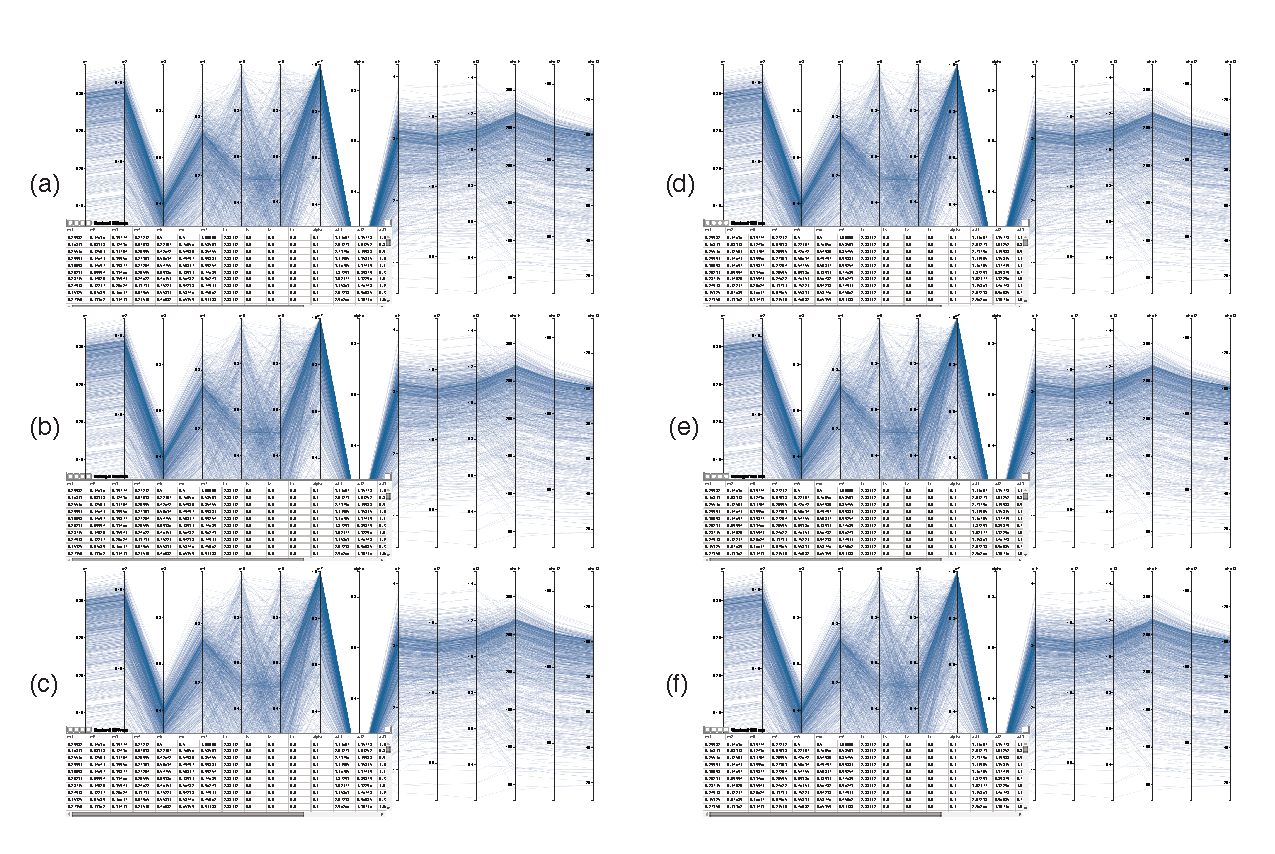
\includegraphics[width=\textwidth]{figs/parcoords.pdf}
\caption{These snapshots show the use of the interactive parallel coordinate visualization of solutions across the activation space. For the task set to 50\% of maximal in the distal direction, we show the
(a) remaining 166 solutions when PI $<$ 60\% 
(b) remaining 57 solutions when DI $<$ 60\%, and the
(c) remaining 57 solutions when we constrain PI $<$ 60\% and DI $<$ 60\%. We also show the
(d) remaining 502 solutions when we select the lower 50\% of $L_1$ costs,
(e) remaining 498 solutions when we select the lower 50\% of $L_2^w$ costs, and the
(f) remaining 220 solutions when we select the lower 50\% across all cost functions in Table \ref{cost_function_tabls} }
\label{fig:parcoords}
\end{figure}

Constraining PI $<$ 60\% still leaves a solution space about three times as large as di $<$ 60\%. 
Observe that constraining DI $<$ 60\% already implies that PI $<$ 60\% as seen in Fig. \ref{fig:parcoords} (b), (c). 
Constraining one muscles does have different effects on the other muscles as for example if ei is constrained below 60\% activation, we see that the bounding box of PI is significantly restricted; however, the same constraint has no effect on the bounding box of EIP.

As there are few steep crossings between $L_1$, $L_2$ and $L_3$, the parallel coordinates suggest correlation of those three cost functions.
Similar correlation is observed for the respective weighted functions.
We provide a scatter plot for their relationships in Appendix Fig. \ref{fig:unweighted_cost_functions} and \ref{fig:weighted_cost_functions}.

% subsection paralleL_coordinates (end)



\subsection*{Changes in the structure of the feasible activation space with increasing force mangitude, a.k.a. how muscle redundancy is lost} % (fold)
\label{sub:activation_spaces_for_increasing_force}
The maximal static fingertip force into any direction (i.e., at $\alpha=1$) is produced by  a unique combination of muscle activations \cite{spoor1983balancing,Chao1978Graphical,valero-cuevas2015fundamentals}. Therefore, the histograms in Fig. \ref{fig:Z_progression} show how the multiple solutions available for sub-maximal forces change and shrink  for increasing force magnitude, from $\alpha=0.1$  to $\alpha=1$. You can track the change in the feasible distributions of a given muscle's activations by following its column from top to bottom ending, naturally, with the unique value needed for maximal force magnitude. 

\begin{figure}[htbp]
\centering
\includegraphics[width=\textwidth]{figs/Z_alphaProgression1430924065026.pdf}
\caption{Distribution of activations in the distal direction and changing force. Each row of histograms uses a Hit-and-Run set. The height of each bar visualizes the percentage of 10,000 solutions found within a given bins that are 0.02 wide (i.e., 2\% of total activation range $[0,1]$).  The shape is as meaningful than the height of individual bins of the histograms. Of note is that the mode of the sub-maximal histograms changes, and is seldom the equivalent of the unique activation value needed to achieve maximal force. The lower- and upper-bounds of the histograms are shown as  vertical dotted lines. [what is that other vertical lines]. To our knowledge this is the first time that the internal structure of the feasible activation set has been visualized.}
\label{fig:Z_progression}
\end{figure}

The solution polytope converges as the difficulty of the task increases; the rate of convergence is different across muscles.
For some muscles the convergence only occurs after $\alpha=0.6$ or $\alpha=0.8$ (as in LUM and EIP), while others converge across the entire progression (e.g.\ DI and PI).
Whereas for example FDS already has a small range of feasible activations at $\alpha=0.1$, EIP has feasible activation $[0,1]$ up to 80\%.

It is imperative to keep in mind that every histogram (regardless of its convergence) is composed of the distribution of all 10,000 points; when the distribution is compressed, the relative percentage of the bars will increase (as evident by the increasing y-axis limits), as we fixed break width ($\Delta x$) to remain constant to 2\% of maximal activation \cite{ball1997elementary}.

The peaks seen in these figures is the perpendicular slice that has the largest relative volume; within the same muscle it does not have to be symmetric between the bounds, and can shift over differing tasks.
As expected, the unique solution at $\alpha=1.0$ appears as a single peak representing 100\% of the sampled points; the bounds and the muscle's unique activation are superimposed.

The most simple finding is that the distributions cannot be inferred by their bounding boxes alone.
Consider the activation distributions between $\alpha = 0.7$ and $\alpha = 0.8$ for LUM, where the median changed by less than 4\% while the lower bound increased by nearly 13\%.
Notably, we observe that a meaningful cross-muscle comparison of point distributions cannot be ascertained by the bounding box. For example, at a task of 10\% of maximal distal force production, EIP and EDC both have lower and upper bounds of 0, and 1, respectively, yet their distributions are thoroughly distinct; the shape of EIP is more symmetric (lower 25\% = 0.36, median = 0.5029, upper 75\% = 0.62), while 75\% of the solutions sampled have EDC higher than 0.74 (see Fig. \ref{fig:Z_progression}).

We find this holds not only for inter-muscle distribution comparisons, but intra-muscular distributions. Consider the significant change in the shape of the distributions across the progression for EDC until the 60\% task; the lower and upper bounds change less than 1\% and 4\%, respectively, while the median shifted by nearly 40\%.
In the most extreme case, the median activation can be exceptionally narrow, while the bounds are wide- for example, EIP at a 90\% task; although activation is bounded between 0.1 and 0.81, approximately 79\% of the solutions exist with EIP activation between just 0.49 and 0.51.

Next, we see that if one muscle had to be fixed throughout the entire force progression, DI and PI would fail; their bounding boxes of tasks below $\alpha=0.4$ do not include the unique solution at $\alpha=1.0$.
We also placed a vertical grey line for the scaled unique solution at maximal force, denoted $\textbf{a}^*$, (e.g. LUM converges to an activation of 1 at maximal distal force, so we put a grey line at 0.8 for $\alpha=0.8$ of maximal distal force).
Since $\alpha \textbf{f}_{\max} = \alpha A \textbf{a}^*$, $\alpha \textbf{a}^*$ is a solution of the feasible activation set at $\alpha$-fraction of the maximal force.
However we observe that for some muscles, these points can lie arbitrarily in the distribution i.e.\ do not have to lie close to the corresponding peaks (e.g.\ musle DI and EIP).




\section{Discussion}
Mostly to be written by Brian
\subsection{Running Time}
The step of the algorithm which are time consuming are finding a starting point, which solves a linear program and can take exponential running time in worst case. For each fixed force vector we only have to find a starting point and an orthonormal basis once, and are hence not of concern for the running time.

Running one loop of the hit and run algorithm only needs linear time, therefore the method will extend to higher dimesions with only linear factor of additinal running time needed.
We thank all of the people.


\bibliographystyle{plain}
\bibliography{redundancyFVC}
%\section{APPENDIX}

\subsection{Finger model data}
$F_o = (123.0, 219.0, 23.52, 91.74,	21.6, 124.8, 129.6)$\\
$
JR = 
\begin{pmatrix}
-0.08941 & -0.0447 & -0.009249 & 0.03669 & 0.1421 & 0.2087 & -0.2138 \\
-0.04689 & -0.1496 & 0.052 &0.052 & 0.0248 & 0.0 & 0.0248 \\ 
0.06472 & 0.001953 & -0.1518 &-0.1518 & 0.2919 & 0.0568 & 0.2067 \\
0.003081 & -0.002352 & -0.0001649 & -0.0001649 & -0.0004483 & 0.0001578 & -0.000685
\end{pmatrix}
$
$task_x = (1.0,0.0,0.0,0.0)$
$task_y = (0.0,1.0,0.0,0.0)$
Palmar force is $task_z = (0.0,0.0,1.0,0.0)$
$task_xy = (1.0,1.0,0.0,0.0)$

\begin{figure}[h]
\centering
\includegraphics[width=0.5\textwidth,page=1]{figs/cost_function_scatterplots.pdf}
\caption{Nonweighted cost functions}
\label{fig:unweighted_cost_functions}
\end{figure}

\begin{figure}[h]
\centering
\includegraphics[width=0.5\textwidth,page=2]{figs/cost_function_scatterplots.pdf}
\caption{Weighted cost functions}
\label{fig:weighted_cost_functions}
\end{figure}

\\
R code to compute the pdf: \\
fixed_db <- the data\\
ecdf(fixed_db[fixed_db['alpha']==0.9,][,3])(c(0.49,0.51))\\
\end{document}
